\documentclass[a4paper,10pt]{article}
\usepackage[T1]{fontenc}
\usepackage[utf8]{inputenc}
\usepackage{lmodern}
\usepackage{indentfirst}
\usepackage{graphicx}
\usepackage{listings}
\usepackage{hyperref}
%\usepackage{fontspec}
%\setmainfont{Ubuntu Mono}

\title{Automated Groceries Storage: Fridge or Non-Fridge decision}

\begin{document}

\maketitle 

\section{Definition}

\subsection{Project Overview}

%Student provides a high-level overview of the project in layman’s terms. Background information such as the problem domain, the project origin, and related data sets or input data is given.

This project is an approximation of detecting if a product should be stored in the fridge or not. \\

Nowadays, time is limited, human have a lot of amount of work to do and thinking in system that could help in everyday tasks is the next step in the human evolution.\\

Some initiatives in Computer Vision and Deep Learning for detecting products were proposed. See "The Freiburg Groceries DataSet" Philipp Jund at el. \cite{freiburgpaper} . Those are focussed in helping big retailers in product storage. \\

This project uses the "Precios Claros" Dataset. It's a public database that store information of retailers products including price, category, picture, etc. Only the images will be used and the objective is based in the product shape determine if it should be stored in the fridge or not.\\


\subsection{Problem Statement}
%The problem which needs to be solved is clearly defined. A strategy for solving the problem, including discussion of the expected solution, has been made.

This project proposes a way to detect if a grocery product should be stored on the fridge or not based on the shape. There are no other works in the field about this problem.\\ 

The solution proposed uses Convolutional Neural Networks. Two approaches were considered: using transfer learning and an original CNN from the scratch.\\

The expectation is that the model build from the scratch could beat in accuracy the pre-trained model.\\

\subsection{Metrics}

At training time, the accuracy will be used to measure the success of the network. Also, the loss and validation loss progress will be checked to provided an accurate model without underfitting or overfitting conditions.\\

The final score will be given by the \textbf{F1-score} over the test dataset. \\

The F1-Score will be calculated using this formula: \\

$F1\_Score = 2 \times \frac{Precision \times Recall}{Precision+Recall}$ \\

The Precision will indicate the percentage of products we are storing correctly in the fridge. The formula will be: \\

$Precision = \frac{Predicted Fridge|Fridge}{Predicted Fridge|Fridge+Predicted Fridge|Non\_Fridge}$ \\

The Recall is going to be definined around the fridge products. We are interested in correctly store them in the fridge and non of them should be out of it. That would lead in the wasting of the product. \\

$Recall = \frac{Predicted Fridge|Fridge}{Predicted Fridge|Fridge+Predicted Non\_Fridge|Fridge}$ \\


\section{Data Exploration}

\subsection{Exploratory Visualization}
% If a dataset is present, features and calculated statistics relevant to the problem have been reported and discussed, along with a sampling of the data. In lieu of a dataset, a thorough description of the input space or input data has been made. Abnormalities or characteristics about the data or input that need to be addressed have been identified.
The Precios Claros Dataset is composed by 4685 images of grocery products. All the images have only 1 product and they have white background. The image is clear.  Each image is RGB and the dimension are 240x240. \\

All the products were classified in fridge or non-fridge according the storage requirements.\\

Some products could be either. For example, a closed soda could be stored in the fridge or not. The criteria in this case is to store it in the fridge. \\

Here are some sample images:

\begin{figure}[ht]
  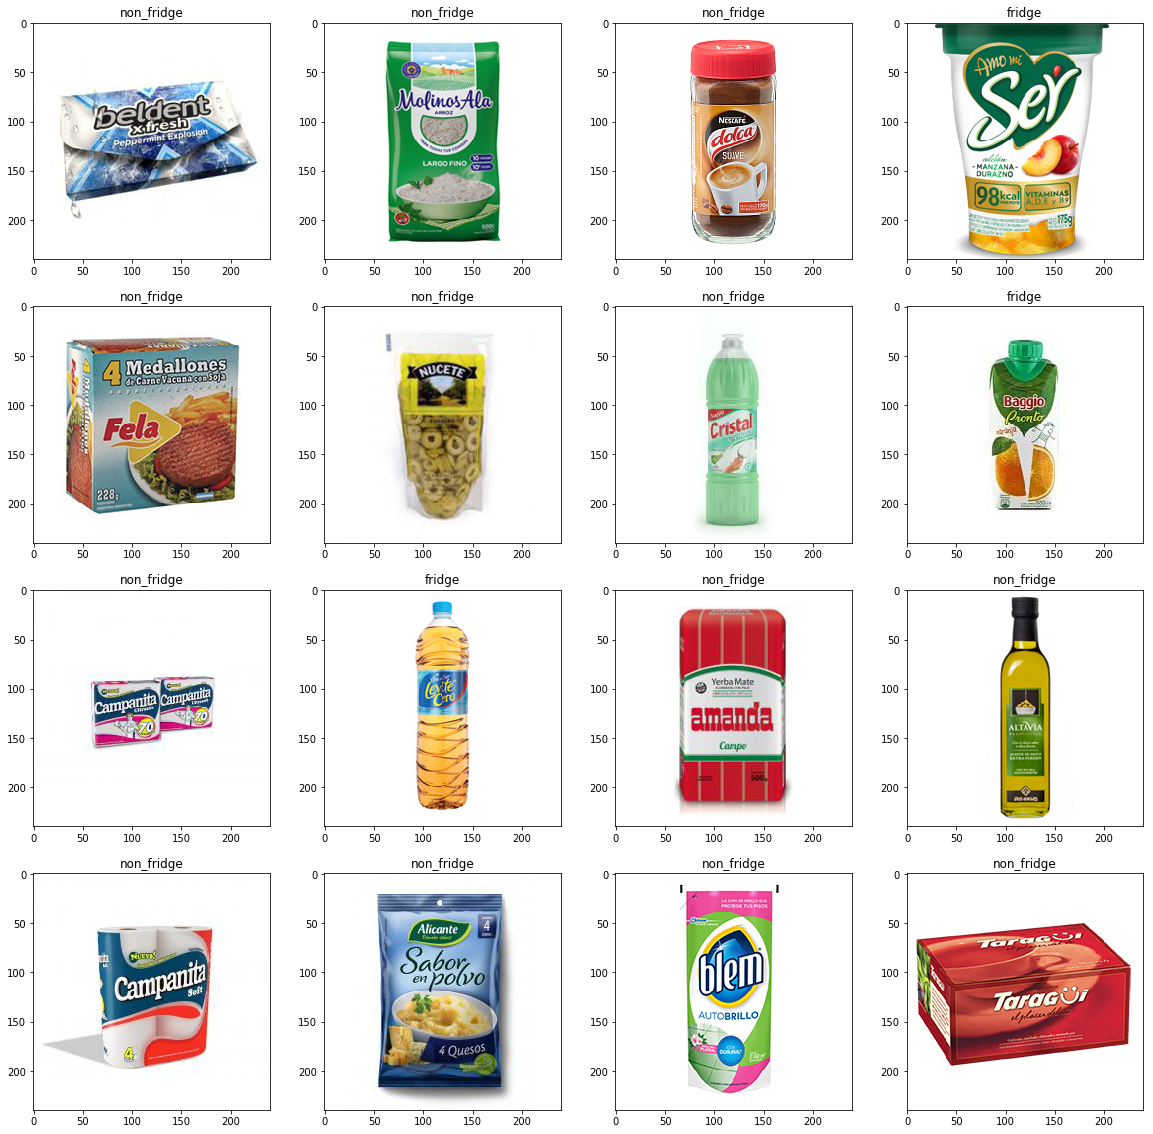
\includegraphics[width=\linewidth]{products2.png}
  \caption{Precios Claros Dataset}
\end{figure}

\newpage

The statistics of the clases is the following:

\begin{figure}[ht]
  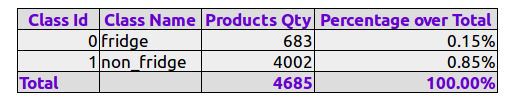
\includegraphics[width=\linewidth]{classes_distribution.png}
  \caption{Precios Claros Classes Distribution}
\end{figure}

\newpage

Notice that most of the products are non-fridge products.

\subsection{Algorithms and Techniques}
% Algorithms and techniques used in the project are thoroughly discussed and properly justified based on the characteristics of the problem.

This project is solved using Deep Learning. The techiques applied are:

\begin{itemize}
  \item Data Augmentation
  \item Transfer Learning
  \item Convolutional Neural Networks
  \item Dropout
  \item Hyperparameters tuning
  \item Optimizer selection
\end{itemize}

\subsubsection{Data Augmentation}

Data Augmentation is a techinique broadly used to prevent overfitting and to increment the training data. The idea is to increment the data by processing the images in the dataset like scales, rotations, etc. \\

For example, if you apply data augmentation over the Precios Claros dataset we can have:

  
\begin{figure}[ht]
  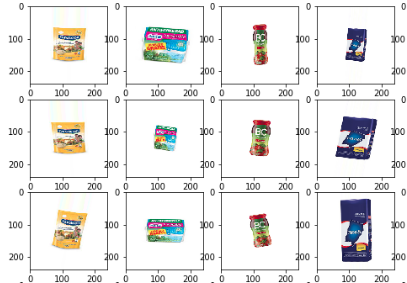
\includegraphics[width=\linewidth]{data_augmentation.png}
  \caption{Data Augmentation}
\end{figure}

\newpage

\subsubsection{Transfer learning}

Transfer learning is a very useful techinique in deep learning that let us use the previous trained model in our data. \\

Models that were trained for weeks and on multiple GPU could be used over new data to make a prediction with amazing results. \\

\subsubsection{Convolutional Neural Networks}

CNN are a kind of Neural Networks mainly used in Computer Vision. It consist in applying convolution operations over an image pixels to create filters that extract different features/characteristic of an image. For example, borders, lines, etc. \\


\subsubsection{Dropout}

Consist in randomly disable some of the units in a Neural Network layer. It uses a probability to decide if the node (unit) needs to be disabled. \\

This will let the NN to not stick to a fixed architecture and don't get stuck in characteristics that can be shared by some nodes. \\
 
\subsubsection{Hyperparameters tuning}

The accuracy of a neural network will depends on different parameters:

\begin{itemize}
  \item Learning Rate
  \item Number of Layers
  \item Batch Size
  \item Number of Units/kernel/strides in the convolutional layer
  \item Dropout probability in the Dropout layers
\end{itemize}

\subsubsection{Optimizer selection}

Optimizer play a fundamental role in learning. The classic Stochastic Gradient Descent algorithm had many improvements. One of them was the adding of momentum, then a Adam, Adamax, and Adagrad new techniques. \\


\subsection{Benchmark}

% Student clearly defines a benchmark result or threshold for comparing performances of solutions obtained.

The Benchmark model is a VGG16 transfer learning model. \\ 

The network structure is defined:  \\

\begin{figure}[h]
  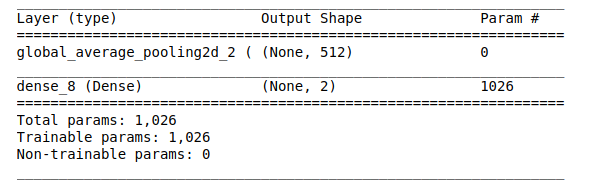
\includegraphics[width=\linewidth]{vgg16_model.png}
  \caption{VGG16 Model}
\end{figure}


The accuracy of the model is: 51.56\%

\begin{center}
\begin{tabular}{ |c|c|c|c| } 
 \hline
       & fridge prediction & no-fridge prediction & total by category \\ 
 \hline
 fridge & 17 & 45 & 62 \\ 
 non-fridge & 17 & 49 & 66 \\ 
 \hline
 Total by prediction & 34 & 94 & \\ 
 \hline
 
\end{tabular}
\end{center}

How many of the products predicted to go to the fridge actually needs to go in the fridge?
Precision: 50.00\% \\

Of the fridge items, how many were correctly predicted
Recall: 27.42\% \\

\noindent\fbox{
\parbox{\textwidth}{
\begin{center}
F1-Score: 0.35
\end{center}
}
}

\section{Methodology}

\subsection{Data Preprocessing}
% All preprocessing steps have been clearly documented. Abnormalities or characteristics about the data or input that needed to be addressed have been corrected. If no data preprocessing is necessary, it has been clearly justified.

The Precios Claros dataset provides 4685 clear images. As it was discussed before Data Augmentation will be used to increase the performance of the Neural Networks. Usually, training over more data allow us to get better results. \\

Also, for using Transfer Learning, the images should be resized (VGG16 uses 224x224x3 images) and the bottleneck extracted. \\

The other preparation required is the separation between train, valid, and test set. \\

The complete pre-processing is summarized in this graph: 
  
\begin{figure}[ht]
  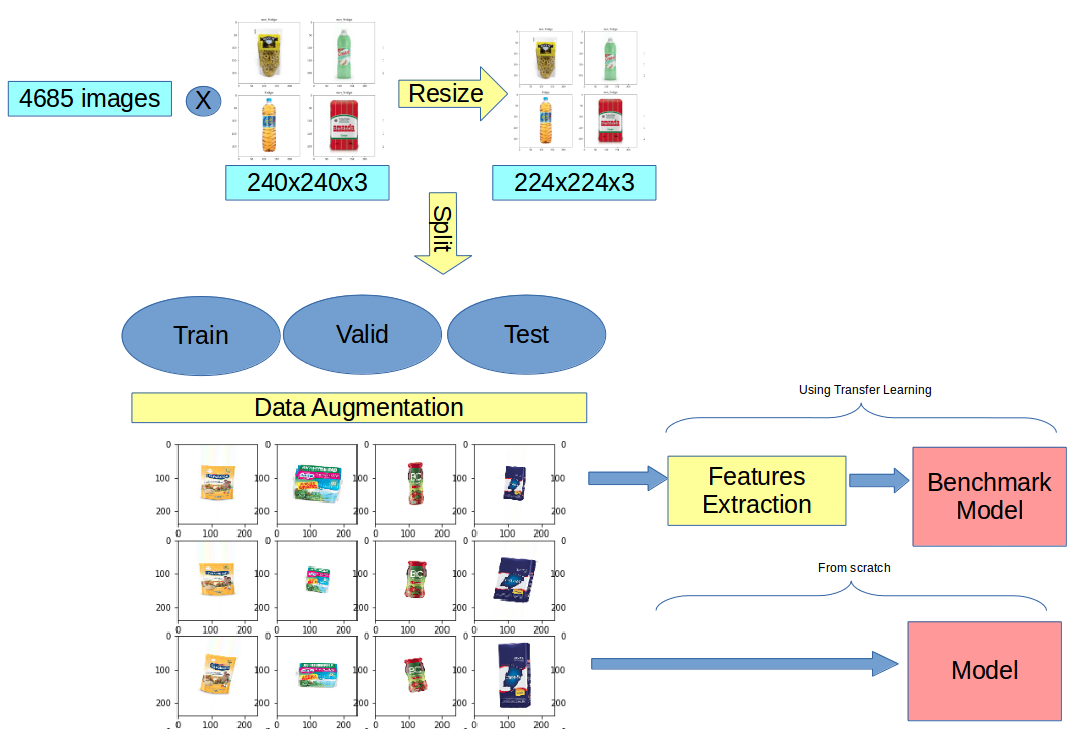
\includegraphics[width=\linewidth]{data_processing.png}
  \caption{Data preparation flow}
\end{figure}

\newpage
\subsection{Implementation}
% The process for which metrics, algorithms, and techniques were implemented with the given datasets or input data has been thoroughly documented. Complications that occurred during the coding process are discussed.

The main issue was the data aumentation implementation. The idea was to generate all the images in memory. The flow method finally allowed me to do that.\\ 


For improving benchmark results, a CNN from the scratch was implemented. The technique uses a Convolutional Neural Network followed by a Max Pooling layer. \\

Dropout layers were used to prevent overfitting. \\ 

\begin{figure}[ht]
  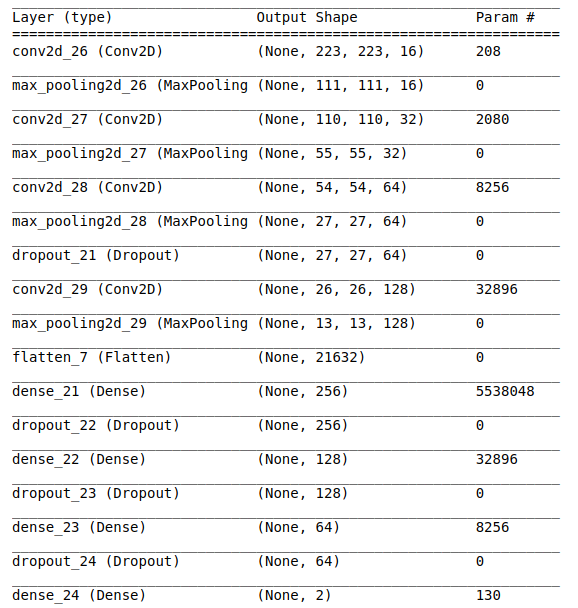
\includegraphics[width=\linewidth]{my_net.png}
  \caption{Data preparation flow}
  \label{fig:boat1}
\end{figure}

\subsection{Refinement}

% The process of improving upon the algorithms and techniques used is clearly documented. Both the initial and final solutions are reported, along with intermediate solutions, if necessary.

The new network was trained for 300 epochs using Model Checkpoint to save the best model weights. \\

The learning rate 0.0001 in Adamax optimizer. Others learning rate, 0.05, 0.01, 0.001 were tried but the best results were in a slow learning. \\

The batch size that best worked was 64. Other values like 32, 128 were tried without outperform the selected parameter value.\\

The optimizer selection was delicate. I first started with a stochastic gradient descent and finally, changes to Adamax that it's an improved optimizer. \\

\section{Results}

\subsection{Model Evaluation and Validation}

% The final model’s qualities — such as parameters — are evaluated in detail. Some type of analysis is used to validate the robustness of the model’s solution.

The accuracy of the model is: 62.32\%

\begin{center}
\begin{tabular}{ |c|c|c|c| } 
 \hline
       & fridge prediction & no-fridge prediction & total by category \\ 
 \hline
 fridge & 29 & 40 & 69 \\ 
 non-fridge & 12 & 57 & 69 \\ 
 \hline
 Total by prediction & 41 & 97 & \\ 
 \hline
 
\end{tabular}
\end{center}

How many of the products predicted to go to the fridge actually needs to go in the fridge?
Precision: 70.73\% \\

Of the fridge items, how many were correctly predicted
Recall: 42.03\% \\

\noindent\fbox{
\parbox{\textwidth}{
\begin{center}
F1-Score: 0.53
\end{center}
}
}


\subsection{Justification}

% The final results are compared to the benchmark result or threshold with some type of statistical analysis. Justification is made as to whether the final model and solution is significant enough to have adequately solved the problem.

The final model is a good aproach to solve the fridge or non-fridge product storage. \\

In the next graph, we are going to compare accuracy, precision, and recall.\\

\begin{figure}[h]
  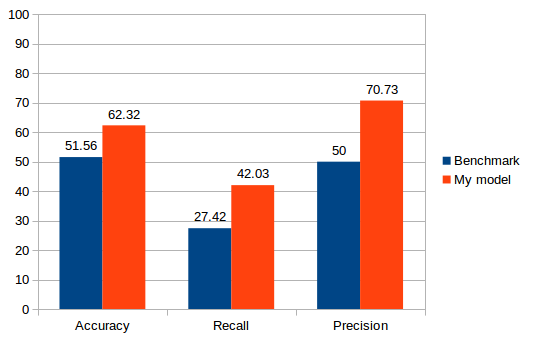
\includegraphics[width=\linewidth]{stats1.png}
  \caption{VGG16 Model}
\end{figure}


All the values were highly improved by the new model. Recall is important to avoid false negative. It's important that we can correctly store all the fridge product. \\

The new model works better and the reason could be related to the dropout layers, and the optimizer chosen. \\ 

Finally, if we compare the F1\_score clearly the new model outperforms the benchmark model. \\ 

\begin{figure}[h]
  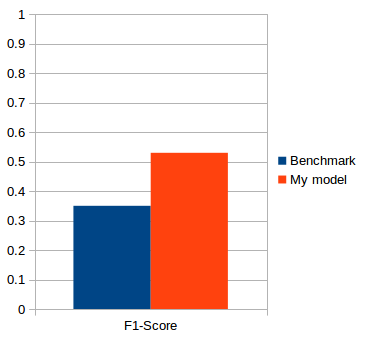
\includegraphics[width=\linewidth]{stats2.png}
  \caption{VGG16 Model}
\end{figure}



\newpage

\section{Conclusion}
 
\subsection{Free-Form Visualization}

% A visualization has been provided that emphasizes an important quality about the project with thorough discussion. Visual cues are clearly defined.


After training, we can review the resutls. They aren't very good.

\begin{figure}[ht]
  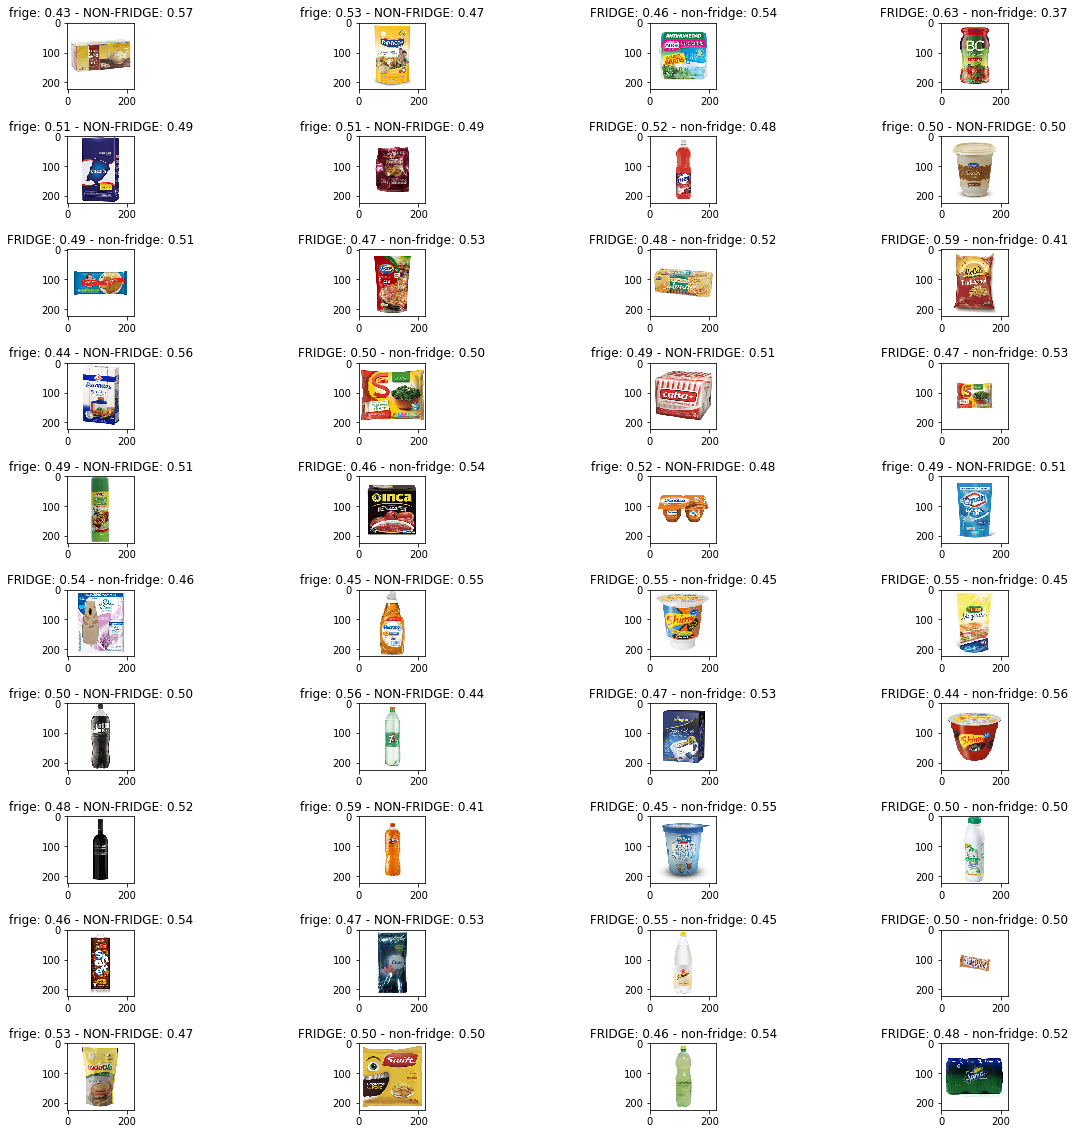
\includegraphics[width=\linewidth]{vgg16_results.png}
  \caption{VGG16 Bechmark Model results - in uppercase the correct label}
\end{figure}

\newpage

They are a little bit better if we consider the new proposed model.
\begin{figure}[ht]
  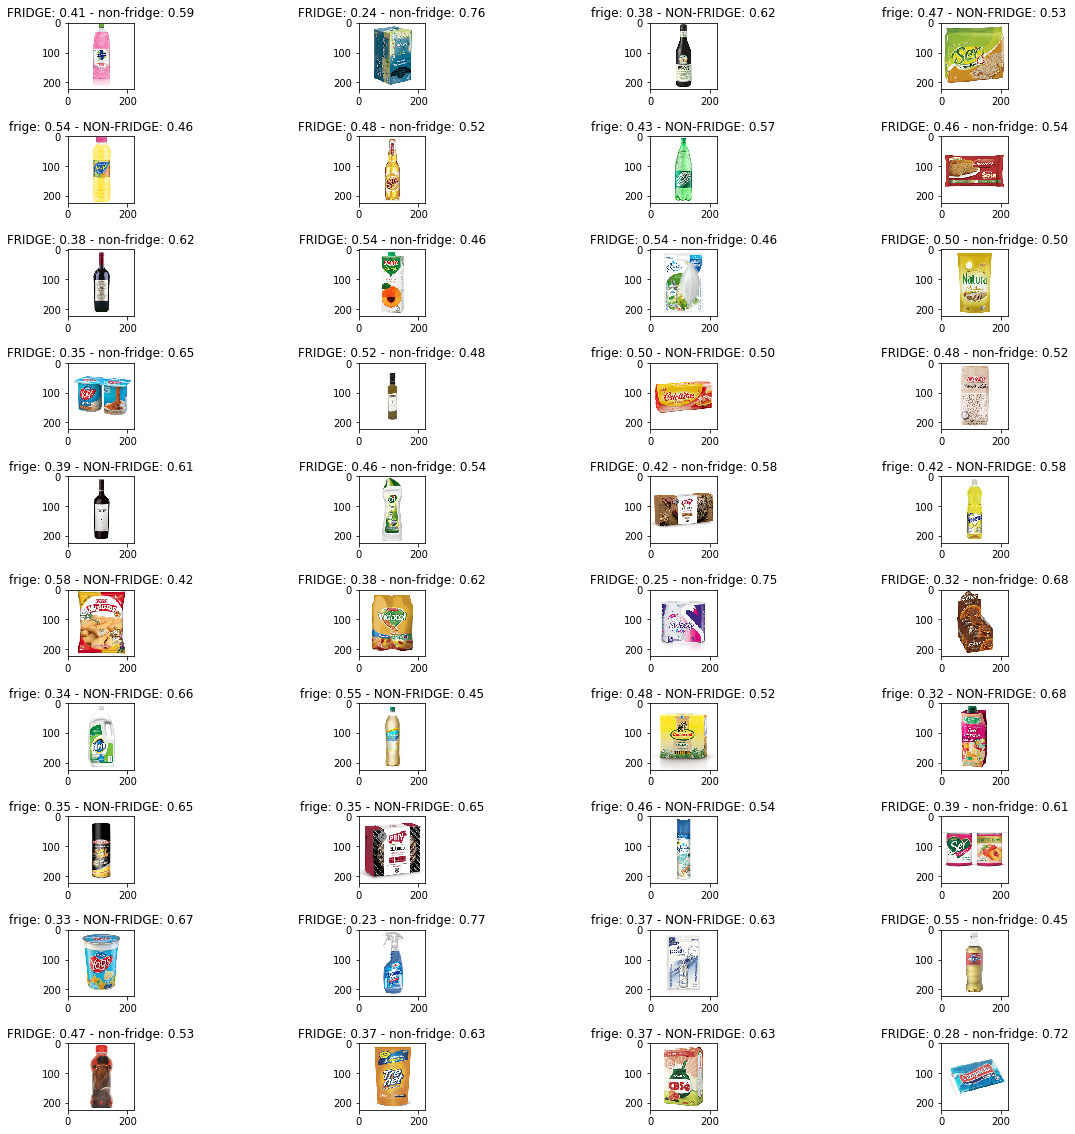
\includegraphics[width=\linewidth]{my_net_results.png}
  \caption{Proposed Model results - in uppercase the correct label}
\end{figure}

\newpage


\subsection{Reflection}

% Student adequately summarizes the end-to-end problem solution and discusses one or two particular aspects of the project they found interesting or difficult.

The solution proposed is better than the benchmark but no better enough. It's important to realize that a product left out of the bridge could be wasted so it's important to have a high accuracy in fridge products. \\

The new model does a good work. If we take a look at the precision, the 70\% of the products that requieres cold will be correctly stored. However, this is not enough. The 30\% of our products will be wasted and that's not good at all. \\


\subsection{Improvement}
% Discussion is made as to how one aspect of the implementation could be improved. Potential solutions resulting from these improvements are considered and compared/contrasted to the current solution.

The problem is hard in its definition. Maybe, just looking the package is not enough information for making a decision. \\

However, the results are quite interesting. A close analysis over the 30\% missclassified fridge products could be performed to develop algorithms that let us increase the accuracy. \\

Also, some transfer learning advanced model could be used like ResNet50 or Xception and compared to the proposed model. 

\begin{thebibliography}{9}
\bibitem{supermarketrobots} 
\textit{Super Market Robots}. 
\url{https://www.fastcodesign.com/90150368/this-online-supermarkets-robots-put-your-order-together-in-minutes} 

\bibitem{preciosclaros} 
\textit{Precios Claros} 
\url{https://www.preciosclaros.gob.ar/\#!/buscar-productos}
 
\bibitem{freiburg} 
\textit{Freiburg groceries dataset} 
\url{http://aisdatasets.informatik.uni-freiburg.de/freiburg\_groceries\_dataset/}

\bibitem{freiburgpaper} 
\textit{Freiburg groceries paper}
\url{https://arxiv.org/abs/1611.05799} 

\bibitem{vgg16}
\textit{VGG16 Paper}
\url{https://arxiv.org/abs/1409.1556}


\end{thebibliography}
 

\end{document}
